\chapter{Classification}
Classification is a most of important task in machine learning. In classification, a function is constructed to determine the category of the input. Generally, the model of classification as following:

The process of classification includes two steps:
\begin{enumerate}
	\item \textbf{Training}: Use the \textbf{training set} to learn what every object of a class looks like. This duration is called training a classifier or learning a model. The training set is a set with the objects which have labeled with specific category.
	\item \textbf{Evaluation}: To evaluate the quality of the classifier. We use a new set \textbf{(test set)} of the objects and try to ask the classifier predict the category of the object in the test set.
\end{enumerate}
In the content of this chapter, we will discuss about the classification techniques, especially, linear classification which technique has used more in neural network and deep learning.
\section{Nearest Neighbour Classifier}
The first approach to Classifier, we will develop Nearest Neighbour Classifier. This classifier do not have any relation with deep learning or convolutional networks, but it will help us to have an overview about classification problem.\\[0.2cm]
The idea of Nearest Neightbour Classifier is comparing each image in test data set with all image in training data set and predict the label of closet training image. And one of simplest methods to compare two images is comparing each pixels of two images and sum of all the differences. Assum that we have two vector \textbf{$I_1$}, \textbf{$I_2$} presented for two images, the equation to compare two images is following (called \textbf{L1 distance}):
\begin{equation}
	d_1(I_1,I,2)=\sum_{p}|{I_1}^p - {I_2}^p|
\end{equation}
Actually, we have many ways to compute the distances between two image. Instead of using L1 distance, we can use \textbf{L2 distance}, which has indicated by square root of euclidean distance between two vectors. The form of L2 distance as: 
\begin{equation}
	d_2(I_1,I,2) = \sqrt{\sum_{p}{({I_1}^p - {I_2}^p)}^2}
\end{equation}
For example, this is a way to compute distace between two images  (fig. \ref{fignncl1}):
\begin{figure}[h]
	\centering
	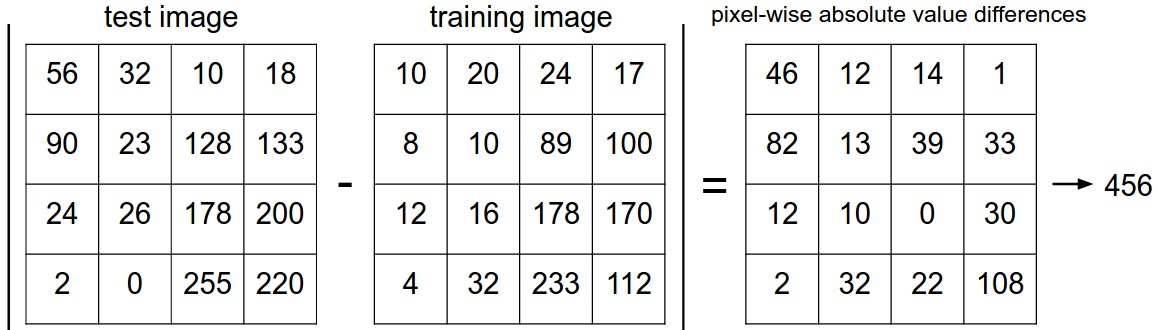
\includegraphics[scale=0.3]{images/nncl1.jpeg}
	\caption{An example used \textbf{L1 distance} to compare two images}
	\label{fignncl1}
\end{figure}
\section{K-Nearest Neighbour Classifier}
In the case of Nearest Neighbour Classifier, we just determine only one closest image in the training data with the test image when we wish to make a prediction. It means that we need some images in training data set that closest with the test image. In this case, we can use the \textbf{k-Nearest Neighbour Classifier}. The idea of this method is finding top \textbf{k} closest images instead of singel closest image (hence, when k = 1, we recover the Nearest Neighbour Classifier).\\[0.2cm]
In practice, what is the best value of k that we should to use? Besides that, we have many choices for  compute the distance between two images different with  L1 distance, L2 distance. The method called \textbf{hyperparameters} is vary for this work. This method comes in the design of many Machine Learning algorithsm, and it is used to choose the setting values. We should try out many different values and  see what works best. This is the idea, but we must be done vary carefully. Another noticed that, we do not try to evaluate on test data set with each \textit{k}. After having the \textit{k}, we evaluate on the test set only a single time, at the end of procedure.\\[0.2cm]
The idea is spitting the training data set in two subsets: the first subset is used to training, the other subset is used to validate (called \textbf{validation set}). The validation set is used as the test set to indicate the value of k. At the end of procedure, we could determine values of k work best. We would then use this value and evaluate once on the actual test set.\\[0.2cm]
In summary, split the training set into training set and validation set. use validation ton tune all hyperparameters. At the end run a single time on the test set and evaluate the result.
\section{Linear Classification}
The (k-)Nearest Neighbour Classifier had introduced about the problem of Image classification, which is predicting the label to an image from a fixed set of labels. But with the these methods, we must spend more time with large datasets an the cost for classifying is expensive. Another classification methods is known as \textbf{linear classification} which is the core of neural networks.
The linear classification has two main components: 
\begin{itemize}
	\item \textbf{Score function}:  which used to map the raw data to score of a category.
	\item \textbf{Loss function}: that quantifies the agreement between predict score and the truth category of the data.
\end{itemize}
The simplest function of a linear mapping is:
\begin{equation}
	y = f(x_i,W,b) = Wx_i + b
\end{equation}
Where:
\begin{itemize}
	\item $x_i$ is the raw data, \textit{example: an image}.
	\item $W$: a matrix parameter, called \textbf{weight} matrix
	\item $b$: vector, called \textbf{bias} vector
	\item $y$: score when consider the data $x_i$ belongs to a category.
\end{itemize}
In equation above, the input image \textbf{$x_i$} is fixed but we can control the setting of parameters \textbf{W and b}. Our goal is setting the parameters that the computing score match with the truth labels of image.
\begin{figure}[h]
	\centering
	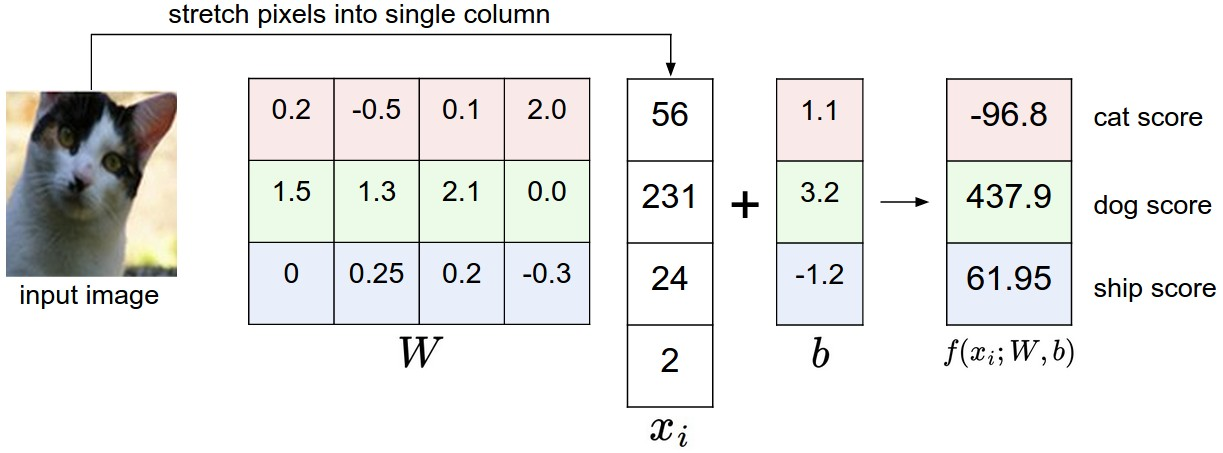
\includegraphics[scale=0.3]{images/lncex}
	\caption{An example of mapping an image to a class scores}
	\label{figlncex}
\end{figure}~\\
In training process, it is a little cumbersome to keep two sets of parameters (W,b) separately. A commonly trick is used to combine two sets of parameters into a single matrix that holds both of them by extending a vector \textbf{$x_i$} with one additional dimension and keep the constant defaut 1. Now, the new score function will be:
\begin{equation}
	y = f(x_i,W,b) = Wx_i
\end{equation}
Visualation of new score function:
\begin{figure}[h]
	\centering
	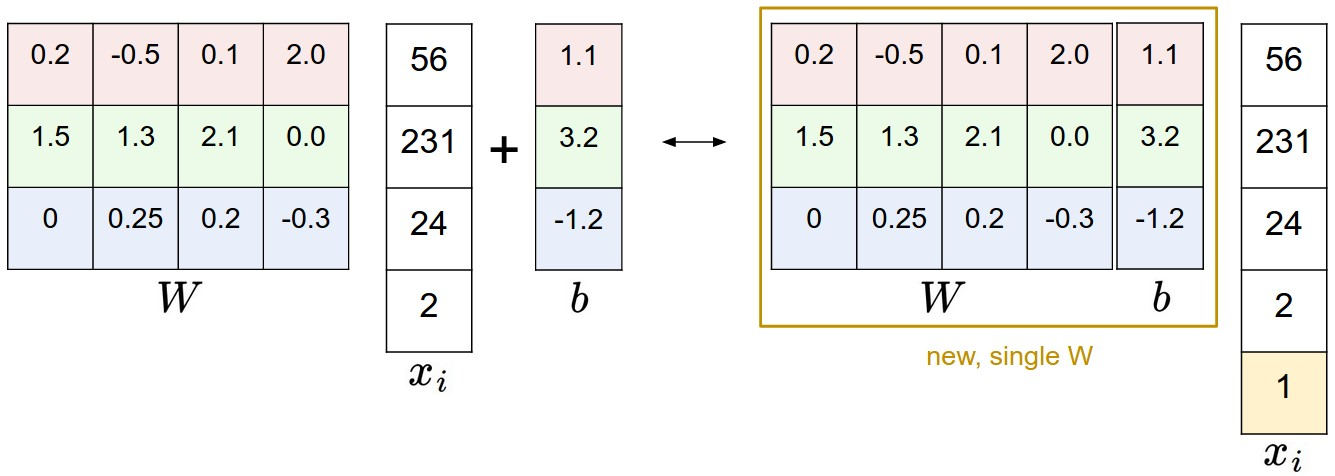
\includegraphics[scale=0.3]{images/lncba}
	\caption{An example of bias trick}
	\label{figlncex}
\end{figure}~\\
As described, we defined a score functions from a pixels value of an image to class scores with set of parameters \textbf{W}. Moreover, we need to control over parameters W such that the class scores are consistent with the ground truth labels in the training data. But not all cases are perfect, the class scores just near with the score of truth labels. So, we are going to measure the wrong with a \textbf{loss function}. Intuitively, the loss will be high if we are doing a poor classifier, ant it will be low if we are doing well. Multicalss Support Vector Machine (SVM) and Softmax function are two commonly methods for this purpose.
\subsection{Multiclass Support Vector Machine loss}
A commonly way to define the loss function called the \textbf{Multiclass Support Vector Machine} (SVM) loss. SVM loss is set up a margin $\Delta$ for the incorrect class scores. It means that SVM loss function wants the score of the correct class to be greater than the incorrect class (predict score) by at leat $\Delta$. If this is not the case, we will accumulate the loss.\\[0.2cm]
The SVM loss for the i-th is formalized as follows:
\begin{equation}
	L_i = \sum_{j \neq y_i }max(0,s_j - s_{y_i} + \Delta)
\end{equation}
Where:
\begin{itemize}
	\item $s_j$ is the score of $x_i$ for j-th class
	\item $s_{y_i}$ is the score of correct class
	\item $\Delta$ is margin 
	\item $max(0,-)$ is thresholding to zero, called hinge loss.
\end{itemize}
For example, we have three predict scores of an image $x_i$ like \textbf{$s = [14,-9,11]$}, and the first class is true class of $x_i$. Assume that $\Delta$ is 10. The SVM loss of this case is following:
\begin{center}
$
	L_i = max(0,-9 - 14 + 10) + max (0,11 - 14 + 10) = 0 + 7 = 7
$
\end{center}
\subsection{Softmax classifer}
The other popular choice to define the loss function  is the \textbf{Softmax classifier}. Unlike SVM which treats the output of score function for each class, the Softmax classifier give a sightly more intuitive output and use the probabilistic description. Instead using theshold zero function as SVM, Softmax is using a \textbf{cross-entropy loss} for \textit{hingle loss}, which has the form.
\begin{equation}
	L_i = -log(\frac{e^{f_{y_i}}}{\sum_j{e^{f_j}}})
	\label{softmax}
\end{equation}
Where: $f_j$ is the j-th element of vector of class scores \textbf{$f$}.\\[0.2cm]
In formula \ref{softmax}, the function $f_j(z) = \frac{e^{z_j}}{\sum_k{e^{z_k}}}$ is called the softmax function. This formula turns the predict scores into probabilistic values (Noticed that sum of all \textbf{$f_j(z) $} is 1).\\[0.2cm]
The cross-entropy between a correct distribution \textbf{p} and an estimated distribution \textbf{q} is defined as:
\begin{equation}
	H(p,q) = -\sum_x{p(x)log(q(x))}
\end{equation}
The Softmax classifier is minimizing the cross-entropy between the estimated socre and true score. At the end, the loss of training process is the average of cross-entropy.
\begin{equation}
	L = \frac{1}{N}\sum_i(H(p,q))
\end{equation}
The image \ref{figsvmsf} describes an example for a comparison between SVM and Softmax:
\begin{figure}[h]
	\centering
	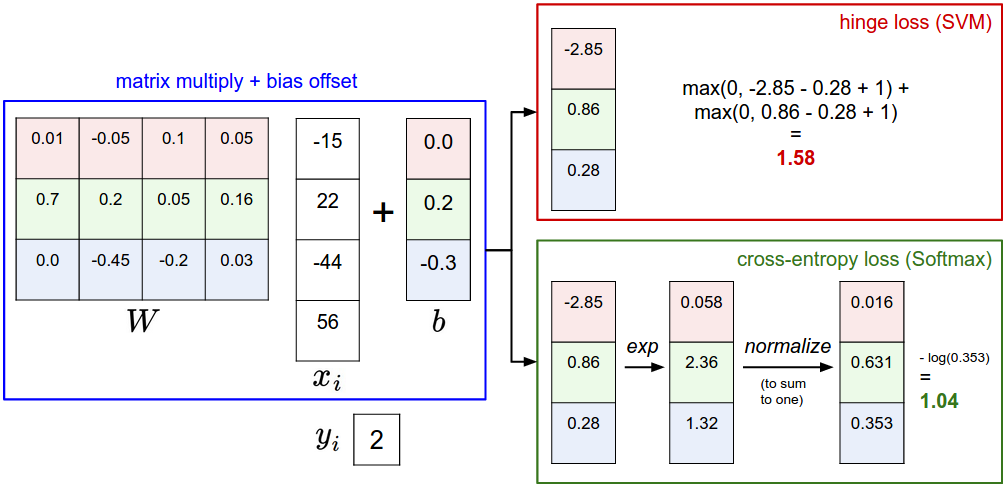
\includegraphics[scale=0.45]{images/svmsf}
	\caption{An example about SVM and Softmax classifiers}
	\label{figsvmsf}
\end{figure}~\\[2.5cm]
Both SVM and Softwax compute the same score of vector f. The difference is the way to present the score f: SVM uses the margin and Softmax uses probabilistic. In practice, the SVM and Softmax are usually used and compared in the machine learning systems.
\section{How to determine the value of W and b?}
\section{Backpropagation}